
\documentclass[
	12pt,				% tamanho da fonte
	openright,			% capítulos começam em pág ímpar (insere página vazia caso preciso)
	oneside,			% para impressão em recto e verso (twoside). Oposto a (oneside)
	a4paper,			% tamanho do papel. 
	chapter=TITLE,		% títulos de capítulos convertidos em letras maiúsculas
	section=TITLE,		% títulos de seções convertidos em letras maiúsculas
	sumario=abnt-6027-2012,
	english,			% idioma adicional para hifenização
	brazil,				% o último idioma é o principal do documento
	fleqn,				% equações alinhadas a esquerda (UDESC/CCT)+
	]{abntex2}

% ----------------------------------------------------------
% Pacotes básicos 
% ----------------------------------------------------------
\usepackage{amsmath}							% Pacote matemático
\usepackage{amssymb}							% Pacote matemático
\usepackage{amsfonts}							% Pacote matemático
%\usepackage{lmodern}							% Usa a fonte Latin Modern		
\usepackage{mathptmx} 							% Usa a fonte Times New Roman	 
\usepackage[T1]{fontenc}						% Selecao de codigos de fonte.
\usepackage[utf8]{inputenc}	
\usepackage{makecell}					% Codificacao do documento (conversão automática dos acentos)
% \usepackage{float}                              % Adiciona o pacote 
\usepackage{lastpage}							% Usado pela Ficha catalográfica
\usepackage{indentfirst}						% Indenta o primeiro parágrafo de cada seção.
\usepackage[dvipsnames,table]{xcolor}			% Controle das cores
\usepackage{graphicx}							% Inclusão de gráficos
\usepackage{microtype} 							% para melhorias de justificação
\usepackage{lipsum}								% para geração de dummy text
\usepackage[brazilian,hyperpageref]{backref}	% Paginas com as citações na bibl
\usepackage[alf,abnt-emphasize=bf,abnt-full-initials=yes]{abntex2cite}					% Citações padrão ABNT
%\usepackage[num]{abntex2cite}					% Citações padrão ABNT numérica
\usepackage{adjustbox}							% Pacote de ajuste de boxes
\usepackage{subcaption}							% Inclusão de Subfiguras e sublegendas		
\usepackage{enumitem}							% Personalização de listas
\usepackage{siunitx}							% Grandezas e unidades
\usepackage[section]{placeins}					% Manter as figuras delimitadas na respectiva seção com a opção [section]
\usepackage{multirow}							% Multi colunas nas tabelas
\usepackage{array,tabularx} 					% Pacotes de tabelas
\usepackage{booktabs} 							% Pacote de tabela profissonal
\usepackage{rotating}							% Rotacionar figuras e tabelas
\usepackage{xfrac}								% Fazer frações n/d em linha
\usepackage{bm}									% Negrito em modo matemático
\usepackage{xstring}							% Manipulação de strings
\usepackage{pgfplots}							% Pacote de Gráficos
\usepackage{tikz}								% Pacote de Figuras
\usepackage[american, cuteinductors,smartlabels, fulldiode, siunitx, americanvoltages, oldvoltagedirection, smartlabels]{circuitikz}						% Pacote de circuitos elétricos
\usepackage{chemformula}						% Pacote para fórmulas químicas
\usepackage{chngcntr}							% Pacte usado para deixar numeração de equações sequencial (UDESC/CCT)
\counterwithout{equation}{chapter}
% fonte: https://latex.org/forum/viewtopic.php?t=15392

% Comando para deixar numeração das equações contínua (1), (2), (3)... ao invés de organizar por capítulos (1.1)(1.2)... (2.1)(2.2)
%\renewcommand{\theequation}{\arabic{equation}}

%\numberwithin{equation}{section}

% Cabecalho cabeçalho somente com numeração de página 10pt
\makepagestyle{PagNumReduzida}
\makeevenhead{PagNumReduzida}{\ABNTEXfontereduzida\thepage}{}{}
\makeoddhead{PagNumReduzida}{}{}{\ABNTEXfontereduzida\thepage}
%fonte: https://github.com/abntex/abntex2/wiki/HowToCustomizarCabecalhoRodape
%fonte: Manual memoir seção 7.3 pg. 111 pdf http://linorg.usp.br/CTAN/macros/latex/contrib/memoir/memman.pdf 

% Personalização das opções das listas
\setlist[itemize]{leftmargin=\parindent}

% Citação online --- MODIFICAR ---
\newcommand{\citeshort}[1]{\citeauthoronline{#1}~(\citeyear{#1})}

\newcommand{\me}[1]{Elaborado pelo autor (#1).}

% Configuração do pgfplots
\pgfplotsset{compat=newest} %compat=1.14
\pgfplotsset{plot coordinates/math parser=false} 
\newlength\figureheight 
\newlength\figurewidth 

% Libraries do TiKz
\usetikzlibrary{quotes,angles,arrows}
\usetikzlibrary{through,calc,math}
\usetikzlibrary{graphs,backgrounds,fit}
\usetikzlibrary{shapes,positioning,patterns,shadows}
\usetikzlibrary{decorations.pathreplacing}
\usetikzlibrary{shapes.geometric}
\usetikzlibrary{arrows.meta}
\usetikzlibrary{external}

%\tikzexternalize[]
%\tikzexternalenable
%\tikzexternalize
%\tikzexternaldisable
%\tikzset{external/force remake}
%\tikzexternalize[shell escape=-enable-write18]

% Configurações do CircuiTiKz
\ctikzset{bipoles/thickness=1}
%\ctikzset{bipoles/length=1.2cm}
\ctikzset{monopoles/ground/width/.initial=.2}
\ctikzset{bipoles/resistor/height=0.25}
\ctikzset{bipoles/resistor/width=0.6}
\ctikzset{bipoles/capacitor/height=0.5}
\ctikzset{bipoles/capacitor/width=0.15}
\ctikzset{bipoles/generic/height=0.25}
\ctikzset{bipoles/generic/width=0.6}
%\ctikzset{bipoles/capacitor polar/length=0.5}
%\ctikzset{bipoles/diode/height=.375}
%\ctikzset{bipoles/diode/width=.3}
%\ctikzset{tripoles/thyristor/height=.8}
%\ctikzset{tripoles/thyristor/width=1}
\ctikzset{bipoles/vsourcesin/height=.5}
\ctikzset{bipoles/vsourcesin/width=.5}
\ctikzset{bipoles/cvsourceam/height=.6}
\ctikzset{bipoles/cvsourceam/width=.6}
%\ctikzset{tripoles/european controlled voltage source/width=.4}

\tikzstyle{every node}=[font=\footnotesize]
\tikzstyle{every path}=[line width=0.25pt,line cap=round,line join=round]
%\tikzstyle{every path}=[line cap=round,line join=round]


% Definição de cores MATLAB
\definecolor{matlab_blue}{rgb}	{         0,    0.4470,    0.7410}
\definecolor{matlab_orange}{rgb}{    0.8500,    0.3250,    0.0980}
\definecolor{matlab_yellow}{rgb}{    0.9290,    0.6940,    0.1250}
\definecolor{matlab_violet}{rgb}{    0.4940,    0.1840,    0.5560}
\definecolor{matlab_green}{rgb}	{	 0.4660,    0.6740,    0.1880}
\definecolor{matlab_lblue}{rgb}	{    0.3010,    0.7450,    0.9330}
\definecolor{matlab_red}{rgb}	{    0.6350,    0.0780,    0.1840}

% Personalização das legendas
\usepackage[format = plain, %hang
			justification = centering,
			labelsep = endash,
			singlelinecheck = false,
			skip = 6pt,
			listformat = simple]{caption}	

% Personalização das unidades
\sisetup{output-decimal-marker = {,}}
\sisetup{exponent-product = \cdot, output-product = \cdot}
\sisetup{tight-spacing=true}
\sisetup{group-digits = false}

% Personalizações de tipo de colunas de tabelas
\newcolumntype{L}[1]{>{\raggedright\let\newline\\\backslash\hspace{0pt}}m{#1}}
\newcolumntype{C}[1]{>{\centering\let\newline\\\arraybackslash\hspace{0pt}}m{#1}}
\newcolumntype{R}[1]{>{\raggedleft\let\newline\\\arraybackslash\hspace{0pt}}m{#1}}

% Personalizações de cores da UDESC
\definecolor{CapaAmareloUDESC}{RGB}{243,186,83}		% Especializacao
\definecolor{CapaVerdeUDESC}{RGB}{0,112,52}			% Mestrado
\definecolor{CapaVermelhoUDESC}{RGB}{171,35,21}		% Doutorado
\definecolor{CapaAzulUDESC}{RGB}{38,54,118} 		% Pós-Doutorado

% CONFIGURAÇÕES DE PACOTES
% Configurações do pacote backref
% Usado sem a opção hyperpageref de backref
\renewcommand{\backrefpagesname}{Citado na(s) página(s):~}
% Texto padrão antes do número das páginas
\renewcommand{\backref}{}
% Define os textos da citação
\renewcommand*{\backrefalt}[4]{
	\ifcase #1 %
	Nenhuma citação no texto.%
	\or
	Citado na página #2.%
	\else
	Citado #1 vezes nas páginas #2.%
	\fi}%

% alterando o aspecto da cor azul
%\definecolor{blue}{RGB}{41,5,195}

% informações do PDF
\makeatletter
\hypersetup{
	%pagebackref=true,
	pdftitle={\@title}, 
	pdfauthor={\@author},
	pdfsubject={\imprimirpreambulo},
	pdfcreator={LaTeX with abnTeX2},
	pdfkeywords={abnt}{latex}{abntex}{abntex2}{trabalho academico}, 
	colorlinks=true,       		% false: boxed links; true: colored links
	linkcolor=black,          	% color of internal links
	citecolor=black,        	% color of links to bibliography
	filecolor=black,      		% color of file links
	urlcolor=black,
	bookmarksdepth=4
}
\makeatother


\makeatletter
\newcommand{\includetikz}[1]{%
	\tikzsetnextfilename{#1}%
	\input{#1.tex}%
}
\makeatother

% ---
% Possibilita criação de Quadros e Lista de quadros.
% Ver https://github.com/abntex/abntex2/issues/176
%
\newcommand{\quadroname}{Quadro}
\newcommand{\listofquadrosname}{Lista de quadros}

\newfloat[chapter]{quadro}{loq}{\quadroname}
\newlistof{listofquadros}{loq}{\listofquadrosname}
\newlistentry{quadro}{loq}{0}

% configurações para atender às regras da ABNT
\setfloatadjustment{quadro}{\centering}
\counterwithout{quadro}{chapter}
\renewcommand{\cftquadroname}{\quadroname\space} 
\renewcommand*{\cftquadroaftersnum}{\hfill--\hfill}

\setfloatlocations{quadro}{hbtp} % Ver https://github.com/abntex/abntex2/issues/176
% ---


% Espaçamento depois do título
\setlength{\afterchapskip}{0.7\baselineskip}
% O tamanho do parágrafo é dado por:
\setlength{\parindent}{1.25cm}
% Controle do espaçamento entre um parágrafo e outro:
\setlength{\parskip}{0.0cm}  % tente também \onelineskip
%\SingleSpacing % Espaçamento simples 
\OnehalfSpacing % Espaçamento 1,5 (UDESC/CCT)
%\DoubleSpacing	% Espaçamento duplo

% ---
% Margens - NBR 14724/2011 - 5.1 Formato
% ---
\setlrmarginsandblock{3cm}{2cm}{*}
\setulmarginsandblock{3cm}{2cm}{*}
\checkandfixthelayout[fixed]
% ---


% To use externalize consider
%https://tex.stackexchange.com/questions/182783/tikzexternalize-not-compatible-with-miktex-2-9-abntex2-package
%Lauro Cesar digged into the problem until he came with a solution for me to test. And it Works!
%
%According to this link:
%
%The package calc changed the commands \setcounter and friends to be fragile. So you have to make them robust. The example below uses etoolbox with \robustify:
%
\usepackage{etoolbox}
\robustify\setcounter
\robustify\addtocounter
\robustify\setlength
\robustify\addtolength


%% How to silence memoir class warning against the use of caption package?
%% https://tex.stackexchange.com/questions/391993/how-to-silence-memoir-class-warning-against-the-use-of-caption-package
%\usepackage{silence}
%\WarningFilter*{memoir}{You are using the caption package with the memoir class}
%\WarningFilter*{Class memoir Warning}{You are using the caption package with the memoir class}

% --------------------------------------------------------
% INICIO DAS CUSTOMIZACOES PARA A UDESC
% --------------------------------------------------------

% --------------------------------------------------------
% Fontes padroes de part, chapter, section, subsection e subsubsection
% --------------------------------------------------------
% --- Chapter ---
\renewcommand{\ABNTEXchapterfont}{\fontseries{b}} %\bfseries
\renewcommand{\ABNTEXchapterfontsize}{\normalsize}
% --- Part ---
\renewcommand{\ABNTEXpartfont}{\ABNTEXchapterfont}
\renewcommand{\ABNTEXpartfontsize}{\LARGE}
% --- Section ---
\renewcommand{\ABNTEXsectionfont}{\normalfont}
\renewcommand{\ABNTEXsectionfontsize}{\normalsize}
% --- SubSection ---
\renewcommand{\ABNTEXsubsectionfont}{\fontseries{b}} %\bfseries
\renewcommand{\ABNTEXsubsectionfontsize}{\normalsize}
% --- SubSubSection ---
\renewcommand{\ABNTEXsubsubsectionfont}{\itshape}
\renewcommand{\ABNTEXsubsubsectionfontsize}{\normalsize}

\renewcommand{\ABNTEXsubsubsubsectionfont}{\normalfont}
\renewcommand{\ABNTEXsubsubsubsectionfontsize}{\normalsize}
% ---

% --------------------------------------------------------
% Fontes das entradas do sumario
% --------------------------------------------------------

\renewcommand{\cftpartfont}{\ABNTEXpartfont\selectfont}
\renewcommand{\cftpartpagefont}{\normalsize\selectfont}

\renewcommand{\cftchapterfont}{\ABNTEXchapterfont\selectfont}
\renewcommand{\cftchapterpagefont}{\normalsize\selectfont}

\renewcommand{\cftsectionfont}{\ABNTEXsectionfont\selectfont}
\renewcommand{\cftsectionpagefont}{\normalsize\selectfont}

\renewcommand{\cftsubsectionfont}{\ABNTEXsubsectionfont\selectfont}
\renewcommand{\cftsubsectionpagefont}{\normalsize\selectfont}

\renewcommand{\cftsubsubsectionfont}{\normalfont\itshape\selectfont}
\renewcommand{\cftsubsubsectionpagefont}{\normalsize\selectfont}

\renewcommand{\cftparagraphfont}{\normalfont\selectfont}
\renewcommand{\cftparagraphpagefont}{\normalsize\selectfont}

% --------------------------------------------------------
% Usando os pacotes hyperref, uppercase... 
% Para deixar a section do toc uppercase precisa de:
% --------------------------------------------------------
\usepackage{textcase}

\makeatletter

\let\oldcontentsline\contentsline
\def\contentsline#1#2{%
	\expandafter\ifx\csname l@#1\endcsname\l@section
	\expandafter\@firstoftwo
	\else
	\expandafter\@secondoftwo
	\fi
	{%
		\oldcontentsline{#1}{\MakeTextUppercase{#2}}%
	}{%
		\oldcontentsline{#1}{#2}%
	}%
}
\makeatother

% --------------------------------------------------------
% Renomenando as entradas de APÊNDICES E ANEXOS
% --------------------------------------------------------

\renewcommand{\apendicesname}{AP\^ENDICES}
\renewcommand{\anexosname}{ANEXOS}


% Manipulação de Strings
%\RequirePackage{xstring}

% Comando para inverter sobrenome e nome
\newcommand{\invertname}[1]{%
	\StrBehind{#1}{{}}, \StrBefore{#1}{{}}%
}%


% --------------------------------------------------------
% Alterando os estilos de Caption e Fonte
% --------------------------------------------------------
\makeatletter
% Define o comando \fonte que respeita as configurações de caption do memoir ou do caption
\renewcommand{\fonte}[2][\fontename]{%
	\M@gettitle{#2}%
	\memlegendinfo{#2}%
	\par
	\begingroup
	\@parboxrestore
	\if@minipage
	\@setminipage
	\fi
	\ABNTEXfontereduzida
	\configureseparator
	\captiondelim{\ABNTEXcaptionfontedelim}
	\@makecaption{#1}{\ignorespaces #2}\par
	\endgroup}


\captionstyle[\raggedright]{\raggedright}

\makeatother

\setlength{\cftbeforechapterskip}{0pt plus 0pt}
\renewcommand*{\insertchapterspace}{}

\newlength{\mylen}	% New length to use with spacing
\setlength{\mylen}{1pt}

\setlength{\cftbeforechapterskip}{\mylen}
\setlength{\cftbeforesectionskip}{\mylen}
\setlength{\cftbeforesubsectionskip}{\mylen}
\setlength{\cftbeforesubsubsectionskip}{\mylen}
\setlength{\cftbeforesubsubsubsectionskip}{\mylen}


% ---
% Ajuste das listas de abreviaturas e siglas ; e símbolos [Personalizada para UDESC com espaçamento 1,5]
% ---

% ---
% Redefinição da Lista de abreviaturas e siglas [Personalizada para UDESC com espaçamento 1,5]
\renewenvironment{siglas}{%
	\pretextualchapter{\listadesiglasname}
	\begin{symbols} 
		\setlength{\itemsep}{0pt}	% Ajuste para Espaçamento 1,5 (UDESC/CCT)
	}{% 
	\end{symbols}
	\cleardoublepage
}
% ---

% ---
% Redefinição da Lista de símbolos [Personalizada para UDESC com espaçamento 1,5]
\renewenvironment{simbolos}{%
	\pretextualchapter{\listadesimbolosname}
	\begin{symbols}
		\setlength{\itemsep}{0pt}	% Ajuste para Espaçamento 1,5 (UDESC/CCT)
	}{%
	\end{symbols}
	\cleardoublepage
}
% ---





% ---
% FIM DAS CUSTOMIZACOES PARA A  Universidade do Estado de Santa Catarina - UDESC/CCT
% ---





	% Incliu pacotes básicos 

% -----------------------------------------------------------------
% Você pode adicionar seus pacotes a partir desta linha;
% -----------------------------------------------------------------

%\usepackage[showframe,pass]{geometry}
%\usepackage[11,12]{pagesel}
\usepackage{float}
\usepackage{hyperref}


% -----------------------------------------------------------------
% Informações de dados para CAPA e FOLHA DE ROSTO
% -----------------------------------------------------------------

\titulo{Trabalho final de Econometria III - Replicação do artigo "Political systems, regime memory, and economic freedom"}%

\autor{Bruno Francisco Schaden \and Yasmin Metzler}%

% ATENÇÃO: O símbolo {} indica o sobrenome para a ficha catalográfica.
% Exemplo: Sherlock Holmes {}da Silva para sobrenomes compostos;
% Exemplo: Arnold Alois {}Schwarzenegger para sobrenome simples.

\instituicao{Universidade do Estado de Santa Catarina, Centro de Ciências Tecnológicas, Programa de Pós--Graduação em Engenharia Elétrica}%

%\tipotrabalho{Tese (Doutorado)}
\tipotrabalho{Trabalho Acadêmico (Econometria III)}

%\preambulo{Tese apresentada ao Programa de Pós--Graduação em Engenharia Elétrica do Centro de Ciências Tecnológicas da Universidade do Estado de Santa Catarina, como requisito parcial para a obtenção do grau de Doutor em Engenharia Elétrica.}

\preambulo{Trabalho final de Econometria III, apresentado ao Curso de Ciências Econômicas da Universidade do Estado de Santa Catarina, como requisito parcial para a obtenção da nota da disciplina.}

\local{Florianópolis}%

\data{\the\year}%
% ---

% compila o indice
\makeindex

% -----------------------------------------------------------------
% Início do documento
% -----------------------------------------------------------------
\begin{document}

\selectlanguage{brazil}
\frenchspacing  % Retira espaço extra obsoleto entre as frases.

% -----------------------------------------------------------------
% ELEMENTOS PRÉ-TEXTUAIS
% -----------------------------------------------------------------
\pretextual

% Você pode comentar os elementos que não deseja em seu trabalho;

% A capa pode ser escolhida dentro do arquivo Capa.tex (TCC, Master, Doc, ...)
% ---
% Capa
% ---


% --------------------------------------------------------
% Capa Padrão
% --------------------------------------------------------
\renewcommand{\imprimircapa}{%
	\begin{capa}%
		\center

		{\fontseries{b}\selectfont\MakeTextUppercase{UNIVERSIDADE DO ESTADO DE SANTA CATARINA -- UDESC}}
		
		{\fontseries{b}\selectfont\MakeTextUppercase{CENTRO DE CIÊNCIAS DA ADMINISTRAÇÃO E SOCIOECONÔMICAS -- ESAG }}
		
		{\fontseries{b}\selectfont\MakeTextUppercase{GRADUAÇÃO -- CIÊNCIAS ECONÔMICAS}}
		
		\vfill
		
		{\fontseries{b}\selectfont\MakeTextUppercase{\normalsize\imprimirautor}}
		
		\vfill
		\begin{center}
			{\fontseries{b}\selectfont\MakeTextUppercase{\imprimirtitulo}}
		\end{center}
		\vfill
		
		\vfill
		
		{\fontseries{b}\selectfont\MakeTextUppercase{\imprimirlocal}}
		\par
		{\fontseries{b}\selectfont \imprimirdata}
		\vspace*{1cm}
	\end{capa}
}



\imprimircapa				% Capa padrão

					% Elemento Obrigatório
% ---
% Folha de rosto
% ---








% --------------------------------------------------------
% folha de rosto 
% --------------------------------------------------------

\makeatletter

\renewcommand{\folhaderostocontent}{
	\begin{center}
		
		{\fontseries{b}\selectfont\MakeTextUppercase{\imprimirautor}}
		
		\vfill
		
		\begin{center}
			{\fontseries{b}\selectfont\MakeTextUppercase{\imprimirtitulo}}
		\end{center}
	
		\vspace*{1.5cm}

		\abntex@ifnotempty{\imprimirpreambulo}{%
			\hspace{.45\textwidth}
			{\begin{minipage}{.5\textwidth}
					\SingleSpacing
					\imprimirpreambulo\par
					\vspace*{4pt}
					{\imprimirorientadorRotulo~\imprimirorientador\par}
					\abntex@ifnotempty{\imprimircoorientador}{%
						{\imprimircoorientadorRotulo~\imprimircoorientador}%
					}%
			\end{minipage}}%
		}%
	
		
		\vfill
		
	{\fontseries{b}\selectfont\MakeTextUppercase{\imprimirlocal}}
	\par
	{\fontseries{b}\selectfont \imprimirdata}
	\vspace*{1cm}
	\end{center}
}


% (o * indica que haverá a ficha bibliográfica)
% ---
\imprimirfolhaderosto
% ---


			% Elemento Obrigatório
% Caso não utilize a Ficha Catalográfica entre na folha de rosto e retire o * de dentro do arquivo FolhadeRosto
% 
% ---
% Inserir a ficha bibliografica
% ---

% Isto é um exemplo de Ficha Catalográfica, ou ``Dados internacionais de
% catalogação-na-publicação''. Você pode utilizar este modelo como referência. 
% Porém, provavelmente a biblioteca da sua universidade lhe fornecerá um PDF
% com a ficha catalográfica definitiva após a defesa do trabalho. Quando estiver
% com o documento, salve-o como PDF no diretório do seu projeto e substitua todo
% o conteúdo de implementação deste arquivo pelo comando abaixo:



% \begin{fichacatalografica}
%     \includepdf{fig_ficha_catalografica.pdf}
% \end{fichacatalografica}


%	\setlength{\parindent}{0cm}
%	\setlength{\parskip}{0pt}
\begin{fichacatalografica}
	%\sffamily
	%\rmfamily
	\ttfamily \hbadness=10000
	\vspace*{\fill}					% Posição vertical
	\begin{center}					% Minipage Centralizado
	Para gerar a ficha catalográfica de teses e \\ 
	dissertações acessar o link:  \\
	https://www.udesc.br/bu/manuais/ficha
	
	\vspace*{8pt}
	
%	\begin{minipage}[c]{8cm}
%	\centering \sffamily
%	 Ficha catalográfica elaborada pelo(a) autor(a), com auxílio do programa de geração automática da Biblioteca Setorial do CCT/UDESC
%	\end{minipage}
	\fbox{\begin{minipage}[c]{12.5cm}		% Largura
	\flushright
	{\begin{minipage}[c]{10.5cm}		% Largura
	\vspace{1.25cm}
	%\footnotesize
	\setlength{\parindent}{1.5em}
	\noindent \invertname{\imprimirautor} \par
	\imprimirtitulo{ }/{ }\imprimirautor. -- \imprimirlocal, \imprimirdata .\par
	\pageref{LastPage} p. : il. ; 30 cm.\par
	\vspace{1.5em}
	\imprimirorientadorRotulo~\imprimirorientador.\par
	\imprimircoorientadorRotulo~\imprimircoorientador.\par
	\imprimirtipotrabalho~--~\imprimirinstituicao, \imprimirlocal, \imprimirdata.\par
	\vspace{1.5em}
		1. Palavra-chave.
		2. Palavra-chave.
		3. Palavra-chave.
 		4. Palavra-chave.
		5. Palavra-chave.
		I. \invertname{\imprimirorientador}.
		II. \invertname{\imprimircoorientador}.
		III. \imprimirinstituicao.
		IV. Título. %
	\vspace{1.25cm}	%		
	\end{minipage}%
	}% 
	\end{minipage}}%
	
	\vspace*{0.5cm}
	
	\end{center}
\end{fichacatalografica}


%\begin{fichacatalografica}
%	\sffamily
%	\vspace*{\fill}					% Posição vertical
%	\begin{center}					% Minipage Centralizado
%	\fbox{\begin{minipage}[c][8cm]{13.5cm}		% Largura
%	\small
%	\imprimirautor
%	%Sobrenome, Nome do autor
%	
%	\hspace{0.5cm} \imprimirtitulo  / \imprimirautor. --
%	\imprimirlocal, \imprimirdata-
%	
%	\hspace{0.5cm} \pageref{LastPage} p. : il. (algumas color.) ; 30 cm.\\
%	
%	\hspace{0.5cm} \imprimirorientadorRotulo~\imprimirorientador\\
%	
%	\hspace{0.5cm}
%	\parbox[t]{\textwidth}{\imprimirtipotrabalho~--~\imprimirinstituicao,
%	\imprimirdata.}\\
%	
%	\hspace{0.5cm}
%		1. Palavra-chave1.
%		2. Palavra-chave2.
%		3. Palavra-chave3.
% 		4. Palavra-chave4.
%		5. Palavra-chave5.
%		I. Orientador.
%		II. Universidade xxx.
%		III. Faculdade de xxx.
%		IV. Título 			
%	\end{minipage}}
%	\end{center}
%\end{fichacatalografica}
% ---

	% Elemento Obrigatório (Verso da Folha)
% 
% ---
% Inserir errata
% ---
\begin{errata}
Elemento opcional. 

Exemplo:

\vspace{\onelineskip}

SOBRENOME, Prenome do Autor. Título de obra: subtítulo (se houver). Ano de depósito. Tipo do trabalho (grau e curso) - Vinculação acadêmica, local de apresentação/defesa, data.

\begin{table}[htb]
\center
\begin{tabular}{|p{2.4cm}|p{2cm}|p{3cm}|p{3cm}|}
  \hline
   \textbf{Folha} & \textbf{Linha}  & \textbf{Onde se lê}  & \textbf{Leia-se}  \\
    \hline
    1 & 10 & auto-conclavo & autoconclavo\\
   \hline
\end{tabular}
\end{table}

\end{errata}
% ---				% Elemento Opcional
% 
% ---
% Inserir folha de aprovação
% ---

% Isto é um exemplo de Folha de aprovação, elemento obrigatório da NBR
% 14724/2011 (seção 4.2.1.3). Você pode utilizar este modelo até a aprovação
% do trabalho. Após isso, substitua todo o conteúdo deste arquivo por uma
% imagem da página assinada pela banca com o comando abaixo:
%
% \includepdf{folhadeaprovacao_final.pdf}
%
\begin{folhadeaprovacao}



	\begin{center}
		{\fontseries{b}\selectfont\MakeTextUppercase{\normalsize\imprimirautor}}
	\end{center}
    \vfill
    
	\vfill
	\begin{center}
		{\fontseries{b}\selectfont\MakeTextUppercase{\imprimirtitulo}}
	\end{center}
	\vfill

    
\abntex@ifnotempty{\imprimirpreambulo}{%
	\hspace{.45\textwidth}
	{\begin{minipage}{.5\textwidth}
			\SingleSpacing
			\imprimirpreambulo\par
			\vspace*{4pt}
			{\imprimirorientadorRotulo~\imprimirorientador\par}
			\abntex@ifnotempty{\imprimircoorientador}{%
				{\imprimircoorientadorRotulo~\imprimircoorientador}%
			}%
	\end{minipage}}%
}%


\vfill
        
	 \begin{center}
	 	
    	{\fontseries{b}\selectfont BANCA EXAMINADORA: }
    	\vspace*{1.75cm}
    
		Nome do Orientador e Titulação \par
		Nome da Instituição
	 \end{center}
	
    {Membros:} 
    
	\begin{center}
		\vspace*{1.25cm}
		Nome do Orientador e Titulação \par
		Nome da Instituição
		
		\vspace*{1.25cm}
		Nome do Orientador e Titulação \par
		Nome da Instituição
		
		\vspace*{1.25cm}
		Nome do Orientador e Titulação \par
		Nome da Instituição

	
	\end{center}
    
    \vspace*{\fill}  
    \begin{center}
    {\imprimirlocal, 01 de maio de \imprimirdata}
	\end{center}
    \vspace*{0.25cm}  
\end{folhadeaprovacao}
% ---




%\textbf{	{Orientador: \vspace{-16pt} }
%	\assinatura{\textbf{Prof. \imprimirorientador , Dr.} \\ Univ. XXX} 
%	{Coorientador: \vspace{-16pt}}   
%	\assinatura{\textbf{Prof. \imprimircoorientador , Dr.} \\ Univ. XXX}
%	
%	{Membros: \vspace{-16pt} } 
%	
%	% --- Exemplo de assinaturas em sequência ---       
%	\setlength{\ABNTEXsignwidth}{8.5cm}
%	
%	\assinatura{\textbf{Prof. Professor, Dr.} \\ Univ. XXX}
%	\assinatura{\textbf{Prof. Professor, Dr.} \\ Univ. XXX}
%	\assinatura{\textbf{Prof. Professor, Dr.} \\ Univ. XXX}
%	
%	% --- Exemplo de assinaturas lado a lado ---
%	\setlength{\ABNTEXsignwidth}{7.5cm}
	%
	%    \noindent\hfill\assinatura*{\textbf{Prof. Professor, Dr.} \\ Univ. XXX}%
	%    \hfill%
	%    \assinatura*{\textbf{Prof. Professor, Dr.} \\ Univ. XXX}%
	%    \hfill
	%    
	%    \noindent\hfill\assinatura*{\textbf{Prof. Professor, Dr.} \\ Univ. XXX}%
	%    \hfill%
	%    \assinatura*{\textbf{Prof. Professor, Dr.} \\ Univ. XXX}%
	%    \hfill}		% Elemento Obrigatório
% ---
% Dedicatória
% ---
\begin{dedicatoria}
   \vspace*{\fill}
%   \begin{flushright}
%   \noindent
%	Este trabalho é dedicado às crianças adultas que,\\
%	quando pequenas, sonharam em se tornar cientistas. 
%   \end{flushright}

{%
	\noindent\hspace{.5\textwidth}
	{\begin{minipage}{.5\textwidth}
			\begin{flushleft}
				Dedico este trabalho ao Professor Rafael Felipe Bressan, cuja habilidade em ensinar Econometria III transformou cada aula em uma verdadeira aventura. Entre momentos de desespero e epifanias matemáticas, obrigado por me ajudar a descobrir que, apesar de todas as adversidades, eu sou mais forte do que imaginava. Afinal, como dizia Muhammad Ali, "Sofra agora e viva o resto da sua vida como um campeão". E, claro, por me mostrar que a econometria, assim como a vida, pode ser vencida com um pouco de coragem e muita persistência.
			\end{flushleft}
	\end{minipage}}%
\vspace*{3cm}
}%

\end{dedicatoria}
% ---
			% Elemento Opcional
% ---
% Agradecimentos
% ---
\begin{agradecimentos}
    Gostaria de expressar minha mais sincera gratidão a todos que me apoiaram ao longo deste semestre, especialmente durante os intermináveis desafios de Econometria III. Quem diria que, em meio a tantos gráficos, fórmulas complexas e noites insones, eu conseguiria sobreviver? A cada aula, eu perdia um pouco mais da minha esperança de entender aquele universo, mas, de alguma forma milagrosa, consegui chegar ao fim.

    Agradeço aos meus remanescentes colegas de classe, que compartilharam comigo o desespero e a luta para decifrar aqueles enigmas econométricos. À minha família e amigos, por me suportarem nos momentos em que eu dizia que nunca conseguiria entender essa disciplina. E, claro, ao café, meu fiel companheiro nas madrugadas de estudo.
    
    Enfim, dedico este trabalho a todos que acreditaram que eu poderia superar Econometria III, mesmo quando eu mesmo duvidava disso. Aos futuros estudantes dessa disciplina, desejo força, pois se eu consegui, talvez qualquer um consegue!

\end{agradecimentos}
% ---		% Elemento Opcional
% ---
% Epígrafe
% ---
\begin{epigrafe}
    \vspace*{\fill}
%	\begin{flushright}
%		\textit{``Eu não falhei, encontrei 10 mil soluções que não davam certo.'' (EDISON, [19--])}
%	\end{flushright}
{%
	\noindent\hspace{.5\textwidth}
	{\begin{minipage}{.5\textwidth}
		\begin{flushright}
			``Eu não falhei, encontrei 10 mil soluções que não davam certo.'' (EDISON, [19--])
		\end{flushright}
	\end{minipage}}%
	\vspace*{3cm}
}%
\end{epigrafe}
% ---				% Elemento Opcional
% ---
% RESUMOS
% ---

% resumo em português
\setlength{\absparsep}{18pt} % ajusta o espaçamento dos parágrafos do resumo
\begin{resumo}
    O artigo "Sistemas políticos, memória de regime e liberdade econômica" de Peter Calcagno, Beatriz Maldonado, Todd Nesbit e Mary Frances Zeager investiga a influência da memória de regimes passados na liberdade econômica de um país. Os autores desenvolvem uma medida inovadora de memória de regime e analisam o efeito geracional de regimes anteriores na liberdade econômica. Por meio de um estudo com 144 países entre 1970 e 2015, o artigo destaca que a memória de regime pode promover melhorias na liberdade econômica em nações historicamente democráticas, enquanto desencoraja em países com histórico autocrático. Esses resultados contribuem para a compreensão de como a cultura, as tradições e as instituições passadas impactam as políticas econômicas atuais.

 \textbf{Palavras-chave}: Sistemas políticos. Memória de regime. Liberdade Econômica. Cultura. Instituições.
\end{resumo}
				% Elemento Obrigatório
% % ---
% Abstract
% ---

% resumo em inglês
\begin{resumo}[Abstract]
 \begin{otherlanguage*}{english}
   Elemento obrigatório para todos os trabalhos de conclusão de curso. Opcional para os demais trabalhos acadêmicos, inclusive para artigo científico. Constitui a versão do resumo em português para um idioma de divulgação internacional. Deve aparecer em página distinta e seguindo a mesma formatação do resumo em português.

   \textbf{Keywords}: Keyword 1. Keyword 2. Keyword 3. Keyword 4. Keyword 5.
 \end{otherlanguage*}
\end{resumo}
				% Elemento Obrigatório

% ---
% inserir lista de ilustrações
% ---
\pdfbookmark[0]{\listfigurename}{lof}
\listoffigures*
\cleardoublepage
% ---

% ---
% inserir lista de quadros
% ---
%\pdfbookmark[0]{\listofquadrosname}{loq}
%\listofquadros*
%\cleardoublepage
% ---


% ---
% inserir lista de tabelas
% ---
\pdfbookmark[0]{\listtablename}{lot}
\listoftables*
\cleardoublepage
% ---

% ---
% inserir lista de abreviaturas e siglas
% ---
\begin{siglas}
	\item[EFW] Economic Freedom of the World (Liberdade Econômica do Mundo)
	\item[PIB] Produto Interno Bruto
	\item[GDP] Gross Domestic Product (Produto Interno Bruto)
	\item[ODA] Official Development Assistance (Assistência Oficial ao Desenvolvimento)
\end{siglas}
% ---

% ---
% inserir lista de símbolos
% ---


\begin{simbolos}
	  \item[$i$] Índice de país
	  \item[$t$] Índice de ano
	  \item[$r$] Índice para o regime
	  \item[$k$] Número de anos desde o término do regime anterior
	  \item[$\text{RegimeMemory}_{it}$] Memória de regime do país \(i\) no ano \(t\)
	  \item[$\text{Polity2}_{(t-1-k)r}$] Pontuação Polity2 do regime \(r\) no ano \(t-1-k\)
	  \item[$w_{(t-1)r}$] Peso do regime \(r\) no ano \(t-1\)
	  \item[$\sum$] Somatório (Soma)
	  \item[$\mathbf{X}_{it-1}$] Vetor de variáveis explicativas controladas no ano \(t-1\)
	  \item[$\boldsymbol{\delta}$] Vetor de coeficientes associados às variáveis explicativas
	  \item[$\Phi_t$] Termo de efeito fixo para o ano \(t\)
	  \item[$\epsilon_{it}$] Termo de erro para o país \(i\) no ano \(t\)
	  \item[$\beta_1$] Coeficiente de regressão da memória de regime
	  \item[$2.5\%$ e $12.5\%$] Taxas de desconto usadas para os resultados principais
\end{simbolos}

% ---
				% Elemento Opcional
% ---
% inserir o sumario
% ---
\pdfbookmark[0]{\contentsname}{toc}
\tableofcontents*
\cleardoublepage
% ---
				% Elemento Obrigatório

% -----------------------------------------------------------------
% ELEMENTOS TEXTUAIS
% -----------------------------------------------------------------
\textual

\pagestyle{PagNumReduzida}						% Comando para cabeçalho somente com numeração de página 10pt
\aliaspagestyle{chapter}{PagNumReduzida}		% Deixar numeração da primeira página com tamanho igual ao resto da numeração
% ref.: https://groups.google.com/g/abntex2/c/CP7g8ZMgi-c/m/KjfEnn5b9a4J


% ---- Mantenha está estrutura, assim você deixa o trabalho mais organizado -------


%\chapter{Introdução}


\section{Do Artigo Científico de Replicação}

O estudo de \cite{https://doi.org/10.1111/coep.12635} explora como sistemas políticos e a memória de regimes anteriores influenciam a liberdade econômica atual. A liberdade econômica é um conceito crítico que afeta o desenvolvimento econômico e social dos países. Este trabalho objetiva replicar os métodos e resultados de \cite{https://doi.org/10.1111/coep.12635} para confirmar a robustez das suas conclusões.

A motivação para esta replicação reside na importância de verificar a reprodutibilidade das pesquisas acadêmicas. Estudos replicados com sucesso reforçam a validade das teorias propostas e aumentam a confiança na literatura científica existente. A abordagem metodológica e os dados utilizados são detalhados nas seções subsequentes.


\subsection{Fonte dos Dados}
Os dados utilizados nesta replicação são provenientes das mesmas fontes mencionadas por \cite{https://doi.org/10.1111/coep.12635}. Utilizamos o dataset replicação composto de liberdade econômica do \cite{fraser2022} e variáveis políticas do \cite{polity2022}. Estes conjuntos de dados fornecem uma cobertura ampla e detalhada de indicadores econômicos e políticos ao longo do tempo.

Adicionalmente, também é incorporado no dataset dados demográficos e econômicos do Banco Mundial para controlar variáveis que possam influenciar a liberdade econômica. Estes dados permitem uma análise comparativa robusta entre diferentes países e regimes ao longo das últimas décadas.

\subsection{Memória de Regime}
A metodologia replicada segue os passos descritos por \cite{https://doi.org/10.1111/coep.12635} somente mudando o softwere de análise de Stata para Python. Utilizamos modelos de regressão linear múltipla para analisar a relação entre sistemas políticos, memória de regime e liberdade econômica. A variável dependente é o índice de liberdade econômica, enquanto as variáveis independentes incluem indicadores políticos e demográficos.

Para capturar os efeitos das mudanças institucionais lentas associadas à mudança de regime, utilizamos duas variáveis para construir nossa medida de memória de regime. Durable é uma variável de contagem que registra o tempo desde a mudança de regime mais recente. Para registrar um efeito na memória de regime, a pontuação máxima de durable para um determinado regime deve ser maior que zero. Polity2 controla o tipo de regime e varia de -10 a 10, com uma pontuação mais baixa indicando um regime mais autocrático e uma pontuação maior indicando um regime mais democrático.

Nossa medida de memória de regime de um país é melhor descrita como uma média ponderada das pontuações de polity2 pelo regime em que os pesos são determinados pela pontuação de durable de cada regime. A construção ampla é descrita da seguinte forma:

\[
\text{RegimeMemory}_{it} = \frac{\sum_{r=0}^{R} \left( w_{(t-1)r} \cdot \text{Polity2}_{(t-1-k)r} \right)}{\sum_{r=0}^{R} w_{(t-1)r}}
\]

onde $i$ e $t$ são índices para país e ano, respectivamente, e $r$ é o índice para o regime. Todas as referências temporais no lado direito são defasadas de modo que a memória de regime não é influenciada diretamente pelas pontuações contemporâneas de polity e durable — ela é destinada a representar puramente a memória dos regimes passados. O subscrito $k$ indexa o número de anos desde o término do regime anterior. Os pesos dos regimes são atribuídos com um valor inicial de um no primeiro ano de existência do regime. A influência desse regime, e portanto seu peso, é assumida como crescente a uma taxa de desconto constante (2,5\% e 12,5\% para os resultados principais apresentados aqui) a cada ano adicional em que o regime está em vigor. Uma vez que um regime termina, o peso atribuído à contribuição desse regime para a memória de regime começa a diminuir na mesma taxa de desconto. Nosso período de amostra para nossa análise de regressão começa em 1970; no entanto, a medida de memória de regime para um determinado país inclui a influência descontada de todos os regimes passados incluídos no conjunto de dados Polity IV.

\begin{figure}[h!]
    \centering
    \caption{Variável de memória de regime para Chile e França entre 1970 e 2015, utilizando taxas de desconto de 2,5\% e 12,5\%, assim como a medida de cálculo alternativa.}
    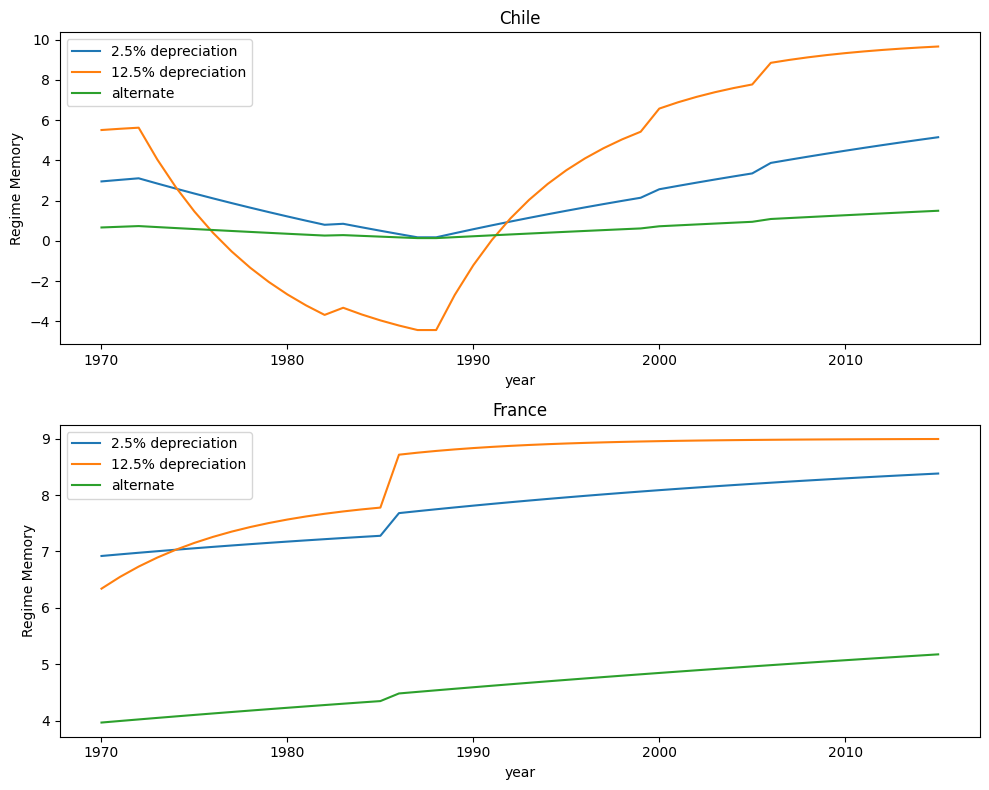
\includegraphics[width=0.8\textwidth]{Textuais/chile.png}
    \fonte{Replicação - Elaborado pelos autores.}
\end{figure}

\subsection{Metodologia Empírica}

A análise de regressão realizada utiliza o modelo de efeitos fixos para examinar a relação entre memória de regime e liberdade econômica. Este modelo permite controlar variáveis não observadas que são constantes ao longo do tempo, mas variam entre os países. A especificação do modelo é dada pela seguinte equação:

\begin{equation}
    \text{EFW}_{it} = \beta_1 \text{RegimeMemory}_{it} + \mathbf{X}_{it-1} \boldsymbol{\delta} + \Phi_t + \epsilon_{it} \quad 
\end{equation}

onde $i$ representa o índice de país e $t$ representa o índice de ano. Para explicar como a memória de regime afeta a liberdade econômica de um país, utilizamos o índice de Liberdade Econômica do Mundo (EFW) do projeto Economic Freedom of the World como nossa medida de liberdade econômica \cite{gwartney2022}. O índice varia de 0 a 10, com pontuações mais baixas denotando menos liberdade econômica e pontuações mais altas denotando mais liberdade.


\section{Resultados}

\subsection{Descrição dos Dados}
As estatísticas descritivas das variáveis foram reproduzidas quase perfeitamente, como mostrado na Tabela \ref{tab:tabela_descritiva}. A diferença encontrada nos números é de ordem de $10^{-2}$, o que é aceitável dada a natureza dos cálculos. A seguir, apresentamos uma breve descrição das variáveis utilizadas na análise:

\begin{itemize}
    \item \textbf{Memória de regime}: Medida que reflete a influência de regimes passados na liberdade econômica atual.
    \item \textbf{Net ODA as \% of GDP}: Ajuda externa líquida como percentual do PIB.
    \item \textbf{Resource rent as \% of GDP}: Renda de recursos como percentual do PIB.
    \item \textbf{ln(GDP per capita)}: Logaritmo do PIB per capita.
    \item \textbf{GDP Growth}: Crescimento do PIB.
    \item \textbf{War Dummy}: Variável indicativa de guerra.
    \item \textbf{Christian Dummy}: Variável indicativa de predominância cristã.
    \item \textbf{British legal origin}: Origem do sistema legal britânico.
    \item \textbf{French legal origin}: Origem do sistema legal francês.
    \item \textbf{Coup d'état}: Variável indicativa de golpes de estado.
    \item \textbf{Gini coefficient}: Coeficiente de Gini.
\end{itemize}

\begin{table}[htbp]
    \centering
    \renewcommand{\arraystretch}{1.1}
    \captionsetup{font=small}
    \caption{Tabela 2 do Artigo Original - Estatísticas Descritivas.}
    \label{tab:tabela_descritiva}
    \small % Ajusta o tamanho da fonte para 10 pontos
    \begin{tabularx}{\textwidth}{l*{8}{>{\raggedleft\arraybackslash}X}}
        \toprule
        \textbf{Variável} & \textbf{N} & \textbf{Média} & \textbf{Desv. Padrão} & \textbf{Mín.} & \textbf{25\%} & \textbf{50\%} & \textbf{75\%} & \textbf{Máx.} \\
        \midrule
        EFW index interpolated & 4697 & 6.14 & 1.30 & 2.37 & 5.18 & 6.20 & 7.18 & 8.85 \\
        EFW index not interpolated & 2534 & 6.53 & 1.16 & 2.37 & 5.75 & 6.65 & 7.44 & 8.85 \\
        2.5\% discount & 4697 & 0.38 & 6.05 & -10.0 & -4.93 & -0.54 & 6.00 & 10.0 \\
        5\% discount & 4697 & 1.01 & 6.34 & -10.0 & -4.84 & 0.79 & 7.00 & 10.0 \\
        7.5\% discount & 4697 & 1.43 & 6.51 & -10.0 & -4.72 & 2.01 & 7.90 & 10.0 \\
        10\% discount & 4697 & 1.73 & 6.64 & -10.0 & -4.65 & 3.03 & 8.03 & 10.0 \\
        12.5\% discount & 4697 & 1.95 & 6.73 & -10.0 & -4.59 & 3.70 & 8.61 & 10.0 \\
        15\% discount & 4697 & 2.10 & 6.79 & -10.0 & -4.63 & 4.00 & 8.89 & 10.0 \\
        Alternative & 4697 & 0.27 & 6.20 & -10.0 & -4.93 & 0.69 & 4.30 & 10.0 \\
        Net ODA as \% of GDP & 4697 & 3.28 & 5.59 & -0.40 & 0.00 & 0.69 & 3.07 & 81.43 \\
        Resource rent as \% of GDP & 4697 & 7.05 & 9.75 & 0.00 & 0.00 & 3.07 & 9.21 & 79.74 \\
        Real GDP per capita & 4697 & 11224.56 & 16503.12 & 157.10 & 1262.87 & 3731.68 & 14263.96 & 114047.91 \\
        GDP growth & 4697 & 3.67 & 4.94 & -50.25 & -4.93 & 0.79 & 7.00 & 39.49 \\
        War Dummy & 4697 & 0.09 & 0.28 & 0 & 0 & 0 & 0 & 1 \\
        Christian Dummy & 4697 & 0.63 & 0.48 & 0 & 0 & 1 & 1 & 1 \\
        UK legal origin & 4697 & 0.30 & 0.46 & 0 & 0 & 0 & 1 & 1 \\
        French legal origin & 4697 & 0.56 & 0.50 & 0 & 0 & 1 & 1 & 1 \\
        Coup d'etats & 4477 & 0.04 & 0.21 & 0 & 0 & 0 & 0 & 1 \\
        Gini & 3530 & 39.07 & 8.84 & 20.30 & 32.40 & 39.60 & 45.07 & 65.40 \\
        \bottomrule
    \end{tabularx}
    \fonte{Elaborado pelos autores.}
\end{table}


\subsection{Reprodução das tabelas do artigo original}

Serão replicadas as tabelas 3, 4, 5 e 6. Estas tabelas os principais resultados das análises empíricas realizadas para investigar a relação entre memória de regime e liberdade econômica. Cada tabela expõe resultados específicos que ajudam a entender como diferentes aspectos dos sistemas políticos e suas mudanças ao longo do tempo influenciam a liberdade econômica em diversos países.

\subsubsection{REPRODUÇÃO DA TABELA 3}

A Tabela 3 apresenta os resultados principais da análise empírica, mostrando como a memória de regime e outros fatores econômicos e políticos influenciam a liberdade econômica, medida pelo índice de Liberdade Econômica do Mundo (EFW). A tabela está dividida em quatro colunas, correspondendo a diferentes especificações do modelo e taxas de depreciação (2,5\% e 12,5\%) da variável de memória de regime.

\begin{itemize}
    \item \textbf{Colunas (1) e (2)}: Essas colunas mostram os resultados utilizando o índice EFW interpolado, que preenche os anos em falta antes de 2000. A memória de regime tem um coeficiente positivo e significativo em ambas as especificações (2,5\% e 12,5\%), indicando que uma maior memória democrática está associada a um aumento na liberdade econômica.
    \item \textbf{Colunas (3) e (4)}: Essas colunas apresentam os resultados sem interpolar o índice EFW, ou seja, utilizando apenas os dados disponíveis a cada cinco anos antes de 2000. Novamente, a memória de regime exibe um impacto positivo e significativo sobre a liberdade econômica, corroborando os resultados encontrados com o índice interpolado.
\end{itemize}

Além da variável principal de interesse (memória de regime), outras variáveis de controle também são incluídas no modelo.

A Tabela 3, portanto, fornece uma visão detalhada de como a memória de regimes passados, bem como uma série de outros fatores econômicos e políticos, influenciam a liberdade econômica de um país. Esses resultados reforçam a importância da história política na determinação das condições econômicas atuais.

\begin{table}
    \caption{Tabela 3 do Artigo Original - Resultados principais.}
    \label{tab:tabela3}
    \small % Ajusta o tamanho da fonte para 10 pontos (que é considerado "small" em LaTeX)
    \begin{tabularx}{\textwidth}{l*{4}{>{\raggedleft\arraybackslash}X}}
        \toprule
        \textbf{Dependent variable} & \makecell[l]{\textbf{EFW index-}\\\textbf{interpolate}\\\textbf{(2.50\%)}} & \makecell[l]{\textbf{EFW index-}\\\textbf{interpolate}\\\textbf{(12.50\%)}} & \makecell[l]{\textbf{EFW}\\\textbf{index}\\\textbf{(2.50\%)}} & \makecell[l]{\textbf{EFW}\\\textbf{index}\\\textbf{(12.50\%)}} \\
        \midrule
        Regime memory & 0.043 & 0.045 & 0.024 & 0.037 \\
        Net ODA as \% of GDP & 0.020 & 0.020 & 0.021 & 0.021 \\
        Resource rent as \% of GDP & -0.023 & -0.021 & -0.028 & -0.024 \\
        ln(GDP per capita) & 0.492 & 0.499 & 0.476 & 0.468 \\
        GDP Growth & 0.019 & 0.019 & 0.021 & 0.020 \\
        War Dummy & -0.234 & -0.209 & -0.195 & -0.200 \\
        Christian Dummy & -0.143 & -0.185 & 0.029 & -0.051 \\
        British legal origin & 0.089 & 0.162 & 0.125 & 0.177 \\
        French legal origin & -0.065 & -0.047 & -0.040 & -0.019 \\
        Number of observations & 4697 & 4697 & 2534 & 2534 \\
        R2 & 0.732 & 0.738 & 0.730 & 0.742 \\
        \bottomrule
    \end{tabularx}
\end{table}


	\subsubsection{REPRODUÇÃO DA TABELA 4 }

	A Tabela 4 apresenta os resultados da análise empírica, incluindo controles adicionais para verificar a robustez dos resultados principais encontrados anteriormente. São incluídas duas variáveis de controle adicionais: golpes de estado e coeficiente de Gini. A tabela está dividida em quatro colunas, correspondendo a diferentes especificações do modelo e taxas de depreciação (2,5\% e 12,5\%) da variável de memória de regime.

	\begin{itemize}
		\item \textbf{Colunas (1) e (2)}: Essas colunas mostram os resultados utilizando o índice EFW interpolado, incluindo a variável de golpe de estado como controle adicional. A memória de regime continua a ter um coeficiente positivo e significativo, indicando que uma maior memória democrática está associada a um aumento na liberdade econômica, mesmo quando consideramos a instabilidade política.
		\item \textbf{Colunas (3) e (4)}: Essas colunas apresentam os resultados com o coeficiente de Gini adicionado como controle adicional. Novamente, a memória de regime exibe um impacto positivo e significativo sobre a liberdade econômica, corroborando os resultados anteriores e mostrando que a desigualdade econômica não altera a relação observada entre memória de regime e liberdade econômica.
	\end{itemize}
	
	A Tabela 4, portanto, reforça a robustez dos achados principais ao incluir variáveis adicionais que controlam por instabilidade política e desigualdade econômica. Esses resultados mostram que a memória dos regimes passados continua a ser um determinante significativo da liberdade econômica, mesmo quando consideradas essas novas variáveis de controle.

	\begin{table}
		\caption{Tabela 4 do Artigo Original - Controles adicionais.}
		\label{tab:tabela4}
		\small % Ajusta o tamanho da fonte para 10 pontos (que é considerado "small" em LaTeX)
		\begin{tabularx}{\textwidth}{l*{4}{>{\raggedleft\arraybackslash}X}}
			\toprule
			\textbf{Dependent variable} & \makecell[l]{\textbf{EFW index-}\\\textbf{interpolate}\\\textbf{(2.50\%)}} & \makecell[l]{\textbf{EFW index-}\\\textbf{interpolate}\\\textbf{(12.50\%)}} & \makecell[l]{\textbf{EFW}\\\textbf{index}\\\textbf{(2.50\%)}} & \makecell[l]{\textbf{EFW}\\\textbf{index}\\\textbf{(12.50\%)}} \\
			\midrule
			Regime memory & 0.045 & 0.046 & 0.045 & 0.050 \\
			Net ODA as \% of GDP & 0.021 & 0.021 & 0.021 & 0.022 \\
			Resource rent as \% of GDP & -0.023 & -0.021 & -0.026 & -0.023 \\
			ln(GDP per capita) & 0.485 & 0.493 & 0.464 & 0.481 \\
			GDP Growth & 0.020 & 0.019 & 0.032 & 0.032 \\
			War Dummy & -0.244 & -0.222 & -0.193 & -0.167 \\
			Christian Dummy & -0.132 & -0.178 & -0.049 & -0.113 \\
			British legal origin & 0.077 & 0.156 & 0.061 & 0.148 \\
			French legal origin & -0.072 & -0.050 & -0.143 & -0.120 \\
			Coup Dummy & -0.039 & -0.021 & -0.131 & -0.102 \\
			Gini Disposable & NA & NA & 0.002 & 0.004 \\
			Number of observations & 4477 & 4477 & 3462 & 3462 \\
			R2 & 0.727 & 0.733 & 0.714 & 0.724 \\
			\bottomrule
		\end{tabularx}
	\end{table}


		\subsubsection{REPRODUÇÃO DA TABELA 5}

		A Tabela 5 apresenta os resultados da análise empírica com defasagens de cinco anos, utilizando diferentes especificações do modelo e taxas de depreciação (2,5\% e 12,5\%) da variável de memória de regime. Esta abordagem permite verificar se as variáveis explicativas têm um impacto retardado sobre a liberdade econômica.

		\begin{itemize}
			\item \textbf{Colunas (1) e (2)}: Essas colunas mostram os resultados utilizando o índice EFW interpolado e defasagens de cinco anos. A memória de regime continua a ter um coeficiente positivo e significativo, indicando que uma maior memória democrática está associada a um aumento na liberdade econômica, mesmo com uma defasagem temporal maior.
			\item \textbf{Colunas (3) e (4)}: Essas colunas apresentam os resultados utilizando defasagens de cinco anos e restringindo a amostra a intervalos de cinco anos. Apesar da redução substancial de amostra, os resultados são robustos, sugerindo que a memória de regime continua a ser um determinante significativo.
		\end{itemize}
		
		A Tabela 5, portanto, reforça a robustez dos achados principais ao utilizar defasagens temporais mais longas e restrições de amostra, demonstrando que a memória dos regimes passados continua a ser um determinante significativo da liberdade econômica, mesmo quando consideradas essas novas abordagens metodológicas.
		

		\begin{table}
			\caption{Tabela 5 do Artigo Original - Defasagens de cinco anos.}
			\label{tab:tabela5}
			\small % Ajusta o tamanho da fonte para 10 pontos (que é considerado "small" em LaTeX)
			\begin{tabularx}{\textwidth}{l*{4}{>{\raggedleft\arraybackslash}X}}
				\toprule
				\textbf{Dependent variable} & \makecell[l]{\textbf{2.50\%}\\\textbf{(1)}} & \makecell[l]{\textbf{12.50\%}\\\textbf{(2)}} & \makecell[l]{\textbf{2.50\%}\\\textbf{(3)}} & \makecell[l]{\textbf{12.50\%}\\\textbf{(4)}} \\
				\midrule
				Regime memory & 0.040 & 0.048 & 0.041 & 0.047 \\
				Net ODA as \% of GDP & 0.020 & 0.021 & 0.024 & 0.025 \\
				Resource rent as \% of GDP & -0.025 & -0.021 & -0.029 & -0.026 \\
				ln(GDP per capita) & 0.433 & 0.437 & 0.471 & 0.488 \\
				GDP Growth & 0.028 & 0.028 & 0.029 & 0.030 \\
				War Dummy & -0.090 & -0.077 & -0.257 & -0.222 \\
				Christian Dummy & 0.021 & -0.048 & -0.069 & -0.131 \\
				British legal origin & 0.062 & 0.128 & 0.068 & 0.144 \\
				French legal origin & -0.175 & -0.151 & -0.138 & -0.121 \\
				Coup d'etat & -0.097 & -0.062 & -0.212 & -0.145 \\
				Gini coefficient & -0.002 & -0.000 & 0.002 & 0.003 \\
				Number of observations & 3097 & 3097 & 727 & 727 \\
				R2 & 0.689 & 0.703 & 0.714 & 0.724 \\
				\bottomrule
			\end{tabularx}
		\end{table}

	\subsubsection{REPRODUÇÃO DA TABELA 6}


A Tabela 6 apresenta os resultados da análise de robustez em subamostras, utilizando diferentes especificações do modelo e taxas de depreciação (2,5\% e 12,5\%) da variável de memória de regime. A análise de subamostras é realizada para verificar se os resultados se mantêm consistentes em diferentes períodos e amostras de países.

\begin{itemize}
    \item \textbf{Colunas (1) e (2)}: Essas colunas mostram os resultados para países com dados disponíveis por 11 ou mais anos. A memória de regime continua a ter um coeficiente positivo e significativo, indicando que uma maior memória democrática está associada a um aumento na liberdade econômica.
    \item \textbf{Colunas (3) e (4)}: Essas colunas apresentam os resultados para países com dados disponíveis por 21 ou mais anos. Novamente, a memória de regime exibe um impacto positivo e significativo sobre a liberdade econômica, corroborando os resultados anteriores.
    \item \textbf{Colunas (5) e (6)}: Essas colunas mostram os resultados para o período de 2000 a 2015, quando o índice EFW foi publicado anualmente. Os resultados indicam que, mesmo nesse período mais recente, a memória de regime continua a ser um determinante significativo da liberdade econômica.
\end{itemize}

A Tabela 6, portanto, reforça a robustez dos achados principais ao utilizar diferentes subamostras e períodos de análise, demonstrando que a memória dos regimes passados continua a ser um determinante significativo da liberdade econômica, mesmo quando consideradas essas novas abordagens metodológicas.


\begin{table}
    \caption{Tabela 6 do Artigo Original - Análise de robustez em subamostras.}
    \label{tab:sub_sample_robustness_check}
    \small % Ajusta o tamanho da fonte para 10 pontos (que é considerado "small" em LaTeX)
    \begin{tabularx}{\textwidth}{l*{6}{>{\raggedleft\arraybackslash}X}}
        \toprule
        \textbf{Dependent variable} & \makecell[l]{\textbf{11 or more}\\\textbf{years}\\\textbf{(2.50\%)}} & \makecell[l]{\textbf{11 or more}\\\textbf{years}\\\textbf{(12.50\%)}} & \makecell[l]{\textbf{21 or more}\\\textbf{years}\\\textbf{(2.50\%)}} & \makecell[l]{\textbf{21 or more}\\\textbf{years}\\\textbf{(12.50\%)}} & \makecell[l]{\textbf{2000-2015}\\\textbf{(2.50\%)}} & \makecell[l]{\textbf{2000-2015}\\\textbf{(12.50\%)}} \\
        \midrule
        Regime memory & 0.047 & 0.051 & 0.050 & 0.051 & 0.012 & 0.030 \\
        Net ODA as \% of GDP & 0.020 & 0.021 & 0.028 & 0.030 & 0.027 & 0.025 \\
        Resource rent as \% of GDP & -0.026 & -0.023 & -0.025 & -0.023 & -0.033 & -0.029 \\
        ln(GDP per capita) & 0.459 & 0.479 & 0.483 & 0.508 & 0.465 & 0.448 \\
        GDP Growth & 0.034 & 0.033 & 0.035 & 0.034 & 0.025 & 0.025 \\
        War Dummy & -0.192 & -0.165 & -0.165 & -0.135 & -0.129 & -0.154 \\
        Christian Dummy & -0.043 & -0.105 & -0.063 & -0.137 & 0.130 & 0.046 \\
        British legal origin & 0.032 & 0.125 & 0.141 & 0.211 & 0.019 & 0.043 \\
        French legal origin & -0.154 & -0.129 & -0.085 & -0.091 & -0.127 & -0.119 \\
        Coup Dummy & -0.126 & -0.100 & -0.124 & -0.095 & -0.136 & -0.128 \\
        Gini Disposable & 0.003 & 0.004 & 0.003 & 0.005 & 0.007 & 0.008 \\
        Number of observations & 3368 & 3368 & 3026 & 3026 & 1814 & 1814 \\
        R2 & 0.715 & 0.726 & 0.722 & 0.729 & 0.697 & 0.708 \\
        \bottomrule
    \end{tabularx}
\end{table}


\section{Conclusão}

A replicação do estudo de \cite{https://doi.org/10.1111/coep.12635} foi realizada com sucesso, confirmando a robustez dos resultados encontrados. Os principais achados do estudo original foram reproduzidos com precisão, demonstrando que a memória de regimes passados tem um impacto significativo sobre a liberdade econômica atual. A análise empírica realizada neste trabalho reforça a importância da história política na determinação das condições econômicas atuais. Esses resultados têm implicações importantes para a compreensão da relação entre política e economia, destacando a influência duradoura dos regimes passados na liberdade econômica de um país. Além disso, esses achados reforçam a importância da replicação de estudos acadêmicos para verificar a validade das teorias propostas e aumentar a confiança na literatura científica existente. Vale ressaltar que, diferentemente da análise original que foi realizada em Stata, a replicação deste estudo foi feita em Python, demonstrando a versatilidade e eficácia dessa linguagem de programação para análises econômicas.
%


\chapter{Desenvolvimento}







%

\chapter{Conclusão}





% -----------------------------------------------------------------
% ELEMENTOS PÓS-TEXTUAIS
% -----------------------------------------------------------------
\postextual

% Você pode comentar os elementos que não deseja em seu trabalho;

% Referências bibliográficas
\bibliography{abntex2-ref_UDESC_2020}	% Elemento Obrigatório

% ----------------------------------------------------------
% Glossário
% ----------------------------------------------------------

%Consulte o manual da classe abntex2 para orientações sobre o glossário.

%\glossary




% ----------------------------------------------------------
% Glossário (Formatado Manualmente)
% ----------------------------------------------------------

\chapter*{GLOSSÁRIO}
\addcontentsline{toc}{chapter}{GLOSSÁRIO}

{ \setlength{\parindent}{0pt} % ambiente sem indentação

\textbf{British legal origin}: Origem do sistema legal britânico.

\textbf{Christian Dummy}: Variável indicativa de predominância cristã.

\textbf{Coup d'état}: Golpe de estado. 

\textbf{Durable}: Variável de contagem que registra o tempo desde a mudança de regime mais recente, usada para medir a memória de regime.

\textbf{EFW (Economic Freedom of the World)}: Liberdade Econômica do Mundo, um índice que mede a liberdade econômica de um país.

\textbf{French legal origin}: Origem do sistema legal francês.

\textbf{GDP (Gross Domestic Product)}: Produto Interno Bruto, o valor total de bens e serviços produzidos em um país.

\textbf{Gini coefficient}: Coeficiente de Gini, uma medida de desigualdade de renda dentro de uma população.

\textbf{ln(GDP per capita)}: Logaritmo do PIB per capita, usado para normalizar a distribuição de dados econômicos.

\textbf{Net ODA as \% of GDP}: Ajuda externa líquida como percentual do PIB, medindo a assistência oficial ao desenvolvimento recebida por um país.

\textbf{Polity2}: Índice que varia de -10 a 10, usado para medir o tipo de regime político de um país, com pontuações mais baixas indicando regimes mais autocráticos e pontuações mais altas indicando regimes mais democráticos.

\textbf{Python}: Linguagem de programação usada para replicar a análise original feita em Stata.

\textbf{RegimeMemory}: Medida de memória de regime, calculada como uma média ponderada das pontuações de Polity2 pelos regimes anteriores, com pesos determinados pela duração do regime.

\textbf{Resource rent as \% of GDP}: Renda de recursos como percentual do PIB, indicando a contribuição da exploração de recursos naturais para a economia.

\textbf{Stata}: Software estatístico usado para análise de dados.

\textbf{War Dummy}: Variável indicativa de guerra, utilizada para identificar períodos de conflito em um país.

} % fim ambiente sem indentação


				% Elemento Opcional

% ----------------------------------------------------------
% Apêndices
% ----------------------------------------------------------

% ---
% Inicia os apêndices
% ---
\begin{apendicesenv}

% Imprime uma página indicando o início dos apêndices
%\partapendices

% ----------------------------------------------------------
\chapter{Países da amostra.}
% ----------------------------------------------------------
\begin{table}[H]
    \caption{Países na amostra}
    \label{tab:sample_countries}
    \small % Ajusta o tamanho da fonte para 10 pontos (que é considerado "small" em LaTeX)
    \begin{tabularx}{\textwidth}{l*{3}{>{\raggedright\arraybackslash}X}}
        \toprule
        \textbf{Country} & \textbf{Country} & \textbf{Country} \\
        \midrule
        Albania & Dominican Republic & Lebanon \\
        Algeria & Ecuador & Lesotho \\
        Angola & Egypt & Liberia \\
        Argentina & El Salvador & Libya \\
        Armenia & Estonia & Lithuania \\
        Australia & Ethiopia & Luxembourg \\
        Austria & Fiji & Macedonia \\
        Azerbaijan & Finland & Madagascar \\
        Bahrain & France & Malawi \\
        Bangladesh & Gabon & Malaysia \\
        Belgium & Gambia & Mali \\
        Benin & Georgia & Mauritania \\
        Bhutan & Germany & Mauritius \\
        Bolivia & Ghana & Mexico \\
        Bosnia and Herzegovina & Greece & Moldova \\
        Botswana & Guatemala & Mongolia \\
        Brazil & Guinea & Morocco \\
        Bulgaria & Guinea-Bissau & Mozambique \\
        Burkina Faso & Guyana & Myanmar \\
        Burundi & Haiti & Namibia \\
        Cambodia & Honduras & Nepal \\
        Cameroon & Hungary & Netherlands \\
        Canada & India & New Zealand \\
        Cape Verde & Indonesia & Nicaragua \\
        Central African Republic & Iran & Niger \\
        Chad & Ireland & Nigeria \\
        Chile & Israel & Norway \\
        China & Italy & Oman \\
        Colombia & Jamaica & Pakistan \\
        Congo, Democratic Republic & Japan & Panama \\
        Congo, Republic & Jordan & Papua New Guinea \\
        Costa Rica & Kazakhstan & Paraguay \\
        Cote d'Ivoire & Kenya & Peru \\
        Croatia & Kuwait & Philippines \\
        Cyprus & Kyrgyz Republic & Poland \\
        Czech Republic & Laos & Portugal \\
        Denmark & Latvia & Qatar \\
        Romania & Russia & Rwanda \\
        Saudi Arabia & Senegal & Sierra Leone \\
        Singapore & Slovak Republic & Slovenia \\
        South Africa & Spain & Sri Lanka \\
        Suriname & Swaziland & Sweden \\
        Switzerland & Syria & Tajikistan \\
        Tanzania & Thailand & Togo \\
        Trinidad and Tobago & Tunisia & UAE \\
        Uganda & Ukraine & United Kingdom \\
        United States & Uruguay & Vietnam \\
        Yemen, Republic & Zambia & Zimbabwe \\
        \bottomrule
    \end{tabularx}
\end{table}

\end{apendicesenv}
% ---				% Elemento Opcional

% ----------------------------------------------------------
% Anexos
% ----------------------------------------------------------
%
% ---
% Inicia os anexos
% ---
\begin{anexosenv}

% Imprime uma página indicando o início dos anexos
%\partanexos

% ---
\chapter{Repositório do Trabalho}
% ---

Para acessar o repositório completo com todos os detalhes de como o trabalho foi feito, visite o seguinte link do GitHub:

\url{https://github.com/Schadenlord/trabalho-final}


\end{anexosenv}
				% Elemento Opcional

%%---------------------------------------------------------------------
%% INDICE REMISSIVO
%%---------------------------------------------------------------------

%\phantompart
%\printindex

%---------------------------------------------------------------------

%%---------------------------------------------------------------------
%% INDICE REMISSIVO (Formatado Manualmente)
%%---------------------------------------------------------------------

\chapter*{ÍNDICE}
\addcontentsline{toc}{chapter}{ÍNDICE}

{ \setlength{\parindent}{0pt}  % ambiente sem indentação
	

Agradecimentos, 6

Análise de robustez em subamostras, 18, 19

Conclusão, 20

Controles adicionais, 16, 17

Dedicação, 4

Descrição dos Dados, 14, 15

Do Artigo Científico de Replicação, 11

Epígrafe, 7

Folha de rosto, 1

Fonte dos Dados, 11

Glossário, 22

Lista de abreviaturas e siglas, 8

Lista de ilustrações, 8

Lista de símbolos, 9

Lista de tabelas, 8

Memória de Regime, 11, 12

Metodologia Empírica, 13

Referências, 21

Resultados, 14

Reprodução das tabelas do artigo original, 15

Reprodução da Tabela 3, 15, 16

Reprodução da Tabela 4, 16, 17

Reprodução da Tabela 5, 17, 18

Reprodução da Tabela 6, 18, 19

Sumário, 10

Título, 1

	
	
	
	
} % fim ambiente sem indentação


		% Elemento Opcional

\end{document}

% -----------------------------------------------------------------
% Fim do Documento
% -----------------------------------------------------------------	